\documentclass[a4paper,chapter,atbegshi]{oblivoir}
\usepackage[dbl4x6]{fapapersize}
\usepackage{amsmath,amssymb,amsfonts}
\usepackage{graphicx,xcolor,caption}
\usepackage{braket,hyperref,nicematrix}
\usepackage{tikz}
\hypersetup{
colorlinks=true,linkcolor=teal,filecolor=magenta,urlcolor=cyan,
}
\newcommand{\comb}[2]{{}_{#1}\mathrm{C}_{#2}}

\title{양자정보학 학습 일지}
\author{김태원}
\date{최초 작성 : 2023년 8월 21일 \\ 최근 편집 : \today}

\begin{document}
\maketitle

\chapter{열역학과 정보}
1824년 프랑스의 물리학자 카르노{\tiny Sadi Carnot}는 열{\tiny heat}이 고온에서
저온으로 떨어질 때만 동력을 얻으며 저온에서 고온으로 올라갈 때는 외부 힘이
필요하다는 결과를 \bnm{열의 동력과 이런 동력을 개발하기 적합한 장치에 관한 
고찰}이라는 책으로 내놓는다. 카르노가 장교로서 증기기관{\tiny steam engine}의
최대 효율을 연구하는 가운데 발견한 결과였다.

지금은 폴란드의 도시인 코샬린 출신 물리학자 클라우지우스{\tiny Rudolf Clausius}는
열이 고온에서 저온으로 떨어질 때만 동력을 얻는다는 카르노의 결과에 동의했다. 
하지만 열이 고온에서 저온으로 떨어질 때 동력의 대상{\tiny body}에 변함이 없다는
가정에는 동의하지 않았다. 즉 열이 고온에서 저온으로 떨어져 동력이 발생할 때 그
대상은 반드시 이전 상태와 다른 상태로 변화한다는 것이다. 순간의 온도 $T$와 열의
극미한 변화량 $\textrm{d}Q$에 대해 아래와 같은 변화량 $\textrm{d}S$였다. 
\begin{equation}
  \textrm{d}S \geq \frac{\textrm{d}Q}{T}
\end{equation}
여기서 클라우지우스는 대상의 상태를 나타내는 함수{\tiny state function} $S$를
`에너지'의 `엔'과 그리스어로 `변환'을 뜻하는 `트로페'{\tiny τροπή}를 따서
\emph{엔트로피\tiny entropy}라고 불렀다. 만약 위 부등식에서 열의 변화량이
대상에 미친 변화량과 일치하여 아래 등식이 성립하면  
\begin{equation}
  \textrm{d}S = \frac{\textrm{d}Q}{T}
\end{equation}
정확히 그만큼 온도를 높여서 대상을 이전 상태로 되돌릴 수 있다. 이처럼
원래대로 되돌릴 수 있는 성질을 \emph{가역\tiny reversible}이라고 부른다.
반면 대상에 미친 변화량이 열의 변화량보다 커서 아래 부등식이 성립하면
\begin{equation}
  \textrm{d}S > \frac{\textrm{d}Q}{T}
\end{equation}
열의 변화량으로 대상에 미친 변화량을 정확하게 추론할 수 없다. 온도를
아무리 조절해도 대상을 원래대로 되돌릴 수 없다는 말이다. 이처럼 원래대로
되돌릴 수 없는 성질을 \emph{비가역}이라고 한다. 정리하면 엔트로피의
변화량이 주어진 온도에 대한 열의 변화량보다 적을 수는 없다. 1865년
클라우지우스는 \snm{역학적 열 이론의 주요 방정식을 간편하게 응용할 수 있는
여러 형태에 관한 고찰}이라는 논문에서 이를 아래처럼 표현한다.
\begin{quote}
  우주의 에너지는 일정하다. \\
  우주의 엔트로피는 최대로 향한다.
\end{quote}
첫 번째 문장에서 `우주'란 대표적인 고립계{\tiny isolated system}다. 우주
바깥에 우주와 상호작용하는 공간이 있다고 하면 우주의 정의와 모순된다. 
따라서 우주는 우주와 상호작용하는 외부를 지니지 않는 고립계다. 그리하여
두 번째 문장은 다음처럼 나타낼 수 있다.
\begin{quote}
  고립계의 엔트로피는 감소하지 않는다.
\end{quote}
이것이 열역학 제2법칙이다.

합스부르크 군주국의 물리학자 볼츠만{\tiny Ludwig 
Boltzmann}은 1877년 \snm{열의 역학적 이론의 두 번째 근본 정리와 열평형 조건에
대한 확률 계산 간의 관계에 관하여}라는 논문에서 엔트로피의 변화량 $\textrm{d}S$가
아니라 엔트로피 $S$ 자체에 주목했다. 논문 제목이 예시하듯 확률이 핵심 도구다. 
확률{\tiny Wahrscheinlichkeit} $W$는 열역학적 계상의 원자들이 배열될 수 있는 
방식의 개수와 동치다. 그리고 엔트로피 $S$는 $W$의 자연로그 $\ln W$에 대해
$k_b$라는 상수로 비례한다. 
\begin{equation}\label{eq:13}
  S=k_B\ln W
\end{equation}
이를테면 구름은 얼음보다 엔트로피가 높다. 왜냐하면 구름 속 물 분자들이
취할 수 있는 미시상태의 개수는 얼음의 구조가 허락하는 것보다 많기 때문이다.

1948년 섀넌{\tiny Claude Shannon}은 \snm{통신의 수학적 이론}이라는 논문에서
디지털계에 볼츠만의 엔트로피 개념을 사용하여 정보이론을 창시한다. 이때 
엔트로피의 단위로 쓰인 볼츠만 상수 $k_B$는 \emph{비트\tiny bit}가 된다. 

1961년 IBM 연구원 란다우어{\tiny Rolf Landauer}는 \snm{컴퓨팅 과정상의 비가역성과
열생성}이라는 논문으로 \emph{란다우어의 원리}를 내놓는다. 란다우어의 원리에 따르면
한 비트의 정보에 대한 비가역 계산에는 어떤 에너지 $E$가 열로 소모되며 $E$는 
적어도 아래와 같다. 
\begin{equation}
  E\geq k_B T \ln 2
\end{equation}
즉 한 비트의 정보를 제거할 때 미시상태의 개수가 $2$와 동치인 엔트로피보다 크거나
같은 엔트로피 증가가 열 에너지 소모의 형태로 나타난다. 

그런데 왜 같은 것도 아니고 크거나 같아야 하는가? 엔트로피의 변화량이 주어진 온도에
대한 열의 변화량보다 큰 경우를 나타낸 공식 \ref{eq:12} ($\textrm{d}S>
\textrm{d}Q/T$)상의 부등호가 비가역성을 가리킨다는 사실을 힌트로 삼으면,
란다우어의 원리가 \emph{비가역적 계산\tiny reversible computation}에 대해 
적용된다고 유추할 수 있겠다. 가령 컴퓨터 및 전자공학도라면 익숙할 NAND 게이트가
있다고 하자. 
\[
  (a,b) \rightarrow \neg(a \wedge b)
\]
두 비트가 입력되고 하나의 비트만 출력되기에 출력 비트로 입력 비트를 복구하는
것은 불가능하다. 비가역적인 셈이다. 또한 입출력 과정에서 하나의 비트가 제거되므로,
란다우어의 원리에 의해 NAND 게이트의 연산에는 적어도 $W=k_BT\ln2$ 만큼의 열이
발생한다. 따라서 수행할 수 있는 계산에는 (컴퓨터가 녹아내린다는) 이론(물리학)적인
한계가 존재한다. 

그러나 1973년 베넷{\tiny Charles Bennett}\footnote{재밌는 사실: 찰스 베넷은 2011년
부경대에 방문했다. \url{https://www.etnews.com/201108210026}}이 
모든 (비가역) 계산을 가역 게이트로 구성할 수 있다는 사실을 보였다. 
실제로 NAND 게이트를 가역으로 구성할 수도 있다. 토폴리{\tiny Toffoli} 게이트를
사용하면 된다. 
\[
  (a,b,c)\rightarrow(a,b,c\oplus a \wedge b)
\]
첫 두 비트가 $1$이면 세 번째 비트를 뒤집고, 그게 아니라면 아무것도
하지 않는 $3$비트 게이트다. 곰곰이 생각하면 NAND와 똑같이 기능하지만 가역이라는
사실을 확인할 수 있다. 그런데 이처럼 모든 (비가역적) 계산을 가역적인 절차로
수행할 수 있다면, 란다우어의 원리의 쓸모란 무엇인가? 

그러자 어디선가 (말 그대로) 악마 하나가 모습을 드러낸다. 이른바 
\emph{멕스웰의 악마}, 1871년 맥스웰{\tiny James Maxwell}이 고안한 사고 실험이다. 

한 상자 속에 기체의 혼합물이 있고, 이 상자에는 $A$와 $B$라는 공간이 있다.
$A$와 $B$는 악마가 열고 닫을 수 있는 문으로 나뉜다. 악마는 두 종류의 기체 분자를
양쪽 공간으로 분리하고자 한다. 악마는 (악마니까 엄청 빨라서) 분자를 하나씩 관찰할
수 있다. 따라서 악마는 문을 조금씩 열고 닫으면서 빠른 분자는 $B$에 몰아넣고 느린
분자는 $A$에 몰아넣는다. 그리하여 상자는 느린 분자의 공간 $A$와 빠른 분자의 공간
$B$로 완벽하게 분리된다. 문제는 악마가 (악마니까 엄청 빨라서) 아무 분자도
건드리지 않은 채 문을 열고 닫았다는 사실이다. 즉 상자는 고립계, 악마와 기체
혼합물이 전혀 상호작용하지 않는 계다. 그런데도 방의 엔트로피가 감소했다.
고립계의 엔트로피는 감소하지 않는다는 열역학 제2법칙이 악마에게 굴복한 꼴이다. 

1982년 베넷은 란다우어의 원리로 악마를 퇴마하고자 했다. 악마가 분자의
\emph{정보를 관측}한다는 사실에 주목하면 된다. 그런데도 앞서 언급한 것처럼 모든
계산은 가역적인 절차로 변환할 수 있으며 관측 또한 계산의 일종이다. 그러니 
이것만으로는 란다우어의 원리에 의해, 즉 비가역적 계산에 대해 비트의 엔트로피보다
크거나 같은 열에너지가 발생하므로 사실 엔트로피는 증가했다고 \emph{말할 수 없다}.

그런데도 란다우어의 원리가 한 발 남았다. 우선 악마 또한 뇌와 같은 기억 공간을
지니기에, 메모리상 제약을 지닌다는 사실에 주목하겠다. 메모리가 다 차서
더는 (가역이든 비가역이든) 계산을 수행할 수 없으면 악마는 어떻게 할 것인가?
\emph{메모리에서 쓸데없는 정보를 지워야 할 것}이다. 정보 제거라는 정보처리를
향해 란다우어의 원리를 쏘면, 한 비트의 정보를 제거할 때 열에너지가 발생한다는
사실에 의해, 엔트로피는 증가한다. 고립계의 엔트로피가 감소하지 않았으므로
열역학 제2법칙을 지켜냈고, 악마를 물리쳤다. 

컴퓨터도 나날이 작아지는데, 란다우어의 원리를 분명하게 고려하지 않으면 화재나
폭발이 발생하리라는 게 교훈이다. 아무튼 이렇듯 물리학의 개념적인 문제를
해결하기 위해 정보 혹은 계산의 개념이 요구된다. 역으로 정보 혹은 계산, 다시 말해
전산학의 문제를 해결하기 위해 물리학, 정확히 말해 양자역학의 개념이 요구되기도
한다. 

\emph{처치-튜링 논제}를 보자. 처치-튜링 논제에 따르면 계산 가능한 함수는 모두
튜링장치로 계산할 수 있다. 즉 모든 컴퓨터는 근본적으로 똑같다. 전산학의
기저를 이루는 근본 (정리가 아니라) 믿음이다. 문제는 \emph{확장 처치-튜링 논제}라는
것이다. 이에 따르면 \emph{효율적으로} 계산 가능한 함수는 모두 튜링장치에 의해
\emph{효율적으로} 계산할 수 있다. 

이 또한 믿음으로, 악마까지는 아니라도 불쾌한 것이라고들 한다. 그런데 양자역학,
정확히 말해 양자정보학은 확장 처치-튜링 논제를 박살낸다. 이 광경을 충분히 묘사할
수 있는 능력을 지니는 것이 양자정보학 학습의 목적 가운데 하나다. 

\chapter{확률론적 모형}


\chapter{새로운 확률론 (작성 중)} 
확률은 익숙하다. 동전을 던진다고 하자. 앞이나 뒤가 나올 것이다. 두 상태의 합은
$1$이고, 각 상태는 $0$ 이상이다. 다시 말해 확률 $P$는 일반적으로 아래와 같다.
\[
  P\in[0,1]
\]
확률 $P$는 $0$ 이상 $1$ 이하인 수라는 뜻이다. 즉 확률이 $101\%$이거나 $-1\%$이라는
말에는 아무 의미가 없다. 대단히 자연스럽다. 하지만 20세기 초 실험과학자들의 눈에
비친 자연은 자연스럽지 않았다. 

그런 실험들은 검색하면 바로 나오니 바로 수학으로 돌격하겠다. ``양자론은 간단히
말해 새로운 유형의 확률론''이라며 시작하는 하디{\tiny Lucien Hardy}의 
논문 {\slshape Quantum Theory From Five Reasonable Axioms}\footnote{ 
\url{https://arxiv.org/abs/quant-ph/0101012}}를 참고한다. 필요한 공리는
다섯 가지다. 
\begin{description}
  \item[공리 1]\emph{확률.} (특정 결과가 관측되는 회수의 비율로 측정한)
    상대빈도{\tiny Relative frequencies}는 주어진 관측이 $n$이 무한이
    되는 극한으로 주어진 $n$개의 계의 
    앙상블{\tiny ensemble}에 대해 수행된 임의의 경우에 대해 같은
    (우리가 확률이라고 부르는) 값을 향한다. 
\end{description}

자연이 자연스럽지 않다는 것을 보인 몇 가지 역사적인 실험들은 생략한다. 대신
21세기의 가장 아름다운 책 가운데 하나가 전하는 이야기를 옮기겠다.
\begin{quote}
  ``양자역학은 확률 이론에서 출발해서 `확률'이라고 부르던 숫자가 음수일 수도
  있도록 일반화하다 보면 필연적으로 등장할 수밖에 없는 이론이다.''
\end{quote}
임의의 사건을 상정하자. 그리고 그 사건에 대한 경우의 수가 $n$이라고 두자.
이 확률은 다음처럼 실수 $n$개로 구성된 벡터로 나타낼 수 있다. 
\[
  \begin{bmatrix}p_1\\\vdots\\p_n\end{bmatrix}
\]
이 벡터에서 수학적으로 주목할 만한 사실은 $p_1,\ldots,p_n$을 모두 합쳐 $1$이
된다는 사실이다. 전문적으로 말해, 확률 벡터의 $1$ 노름{\tiny norm}은 $1$이다.
여기서 노름이란 크기와 같은 뜻이며, $1$ 노름이란 각 항목의 $1$승을 모두 더했다는 
뜻이다. 

$1$ 노름이 있다면 또 무엇이 있겠는가? $2$ 노름이 있다. $2$ 노름이란 각 항목의
제곱을 모두 더한 것의 제곱근이다. 그렇다면 확률론이 $1$ 노름이 아니라 $2$ 노름을
적용할 수 있을까? 그렇다고 하자. $2$ 노름 벡터로 비트를 표현하면 아래와 같다.
\begin{equation}
  (\alpha,\beta):\sqrt{\alpha^2+\beta^2}=1
\end{equation}
그리고 이는 원의 방정식으로 익숙한 $\alpha^2+\beta^2=1$이다.  
\begin{center}
  \begin{tikzpicture}
    \draw[fill=none](0,0)circle(1.0); 
    \draw[](0,-1.3)--(0,1.5) node[above]{$\beta$};
    \draw[](-1.5,0)--(1.5,0) node[right]{$\alpha$};
  \end{tikzpicture}
\end{center}
여기 \emph{관측\tiny observation}이라는 개념을 도입한다. 관측 결과는 $0$이나
$1$이다. 이렇게 주어진 벡터 $(\alpha,\beta)$에서 두 수의 합이 $1$이 되도록
하려면 어떻게 할 것인가? 간단하다. $0$을 볼 확률을 $\alpha^2$으로, 
$1$을 볼 확률을 $\beta^2$으로 정한다.

동전을 던질 때, 동전이라는 계는 자신을 둘러싼 환경과 상호작용한다. 그리고 인간은
입자와 상호작용을 직관으로 분리할 수 없다. 그래서 자연스러워 보인다. 
잘 알려진 것처럼 슈뢰딩거 씨의 고양이는
상자를 열면 죽었거나 살아있다. 직관으로는 고양이의 생과 사라는 상태의 
\emph{중첩\tiny superposition}이 관측되지 않는다. 왜냐하면 고양이가 끊임없이 
주변 환경과 상호작용하기 때문이다. 중첩은 입자를 제 환경에 대해 고립시켜야
가능하다. 양자컴퓨터라는 물건을 만들기 어려운 이유가 이것이다. 입자를 환경에서
격리하는 일 자체가 어렵다. 

(필자는 고등학교를 다니지 않아서 모르겠지만) 고교 과학 시간에 나오는 것처럼
핵을 중심으로 회전하는 전자가 있다고 하자. 20세기 초 과학자들은 전자가 에너지를
상실하며 핵과 충돌할 때까지 나선 운동을 한다고 봤다. 문제는 전자의 궤도가
안정적이라는 사실이다. 그리고 이런 안정성과 이중 슬릿 실험을 비롯한 결과들을
설명하기 적합한 도구는 고전적인 확률론이 아니라 \emph{진폭\tiny amplitude}이었다.

앞서 언급한 것처럼 고전적인 확률은 $P\in[0,1]$, 다시 말해 $101\%$나 $-1\%$ 같은
확률이 존재할 수는 없다. 그런데 진폭 $\alpha$는 복소수다. 또 \emph{보른 규칙}에
따르면 특정 결과를 보는 확률은 진폭의 절댓값을 제곱한 것과 같다. 보른 규칙은
양자역학의 핵심 가정으로, 보른{\tiny Max Born}이 1926년 슈뢰딩거 방정식의
파동함수를 해석하는 가운데 내놓았다. 보른 규칙이 핵심적인 이유는 이 규칙이
실험 결과와 딱 들어맞는 `해석'이기 때문이다. 여기에 엄청난 세계관이 담긴 것은
아니고 아무튼 정말 딱 들어맞기 때문이다. (이를 `코펜하겐 해석'이라고 부른다)
\begin{equation}\label{eq:11}
P=|\alpha|^2
\end{equation}
보른 규칙 \ref{eq:11}을 사용해 이중 슬릿 실험을 전개해 보자. 우선 $\alpha$를 
광자가 스크린상의 특정 지점에 부딪히는 총 진폭이라고 하자. 그리고 $\alpha_1$은
1번 슬릿만 열린 경우 부딪히는 진폭, $\alpha_2$는 2번 슬릿만 열린 경우 부딪히는
진폭이라고 하자. 보른 규칙 \ref{eq:11}에 따르면 두 슬릿 모두 열린 경우
광자가 특정 지점에 부딪히는 확률 $P$는 아래와 같다.
\begin{align*}
  P &= |\alpha|^2 \\ 
    &= |\alpha_1+\alpha_2|^2 \\ 
    &= |\alpha_1|^2 + |\alpha_2|^2 + \overline{\alpha_1}\alpha_2+\alpha_1\overline{\alpha_2}
\end{align*}
$\alpha_1=\frac{1}{2},\alpha_2=-\frac{1}{2}$의 진폭으로 두 슬릿이 모두 열리면
$P=0$이지만 둘 중 하나의 슬릿만 열리면 $P=\frac{1}{4}$로, 경우의 수를 늘리니까
오히려 확률이 줄어든 셈이다. 이중 슬릿 실험과 딱 맞는 결과이며, 이는 전자의 
나선 궤도가 안정적인 이유와 같다. 어떤 경로는 양의 진폭을 지니고 어떤 경로는
음의 진폭을 지녀 서로 소거하는 것이다. 이런 현상을 \emph{간섭\tiny
interference}이라고 부른다.  

진폭을 다루려면 복소행렬 혹은 어떤 특별한 변환들이 필요하다. 가령 아래 $4\times 4$
행렬은 통제된 NOT 혹은 CNOT이라고 부르는 변환이다. 
\begin{equation}
  \textrm{CNOT } = 
  \begin{bNiceMatrix}[first-col, first-row]
    & \scriptstyle00 & \scriptstyle01 & \scriptstyle10 & \scriptstyle11 \\
    \scriptstyle00 & 1 & 0 & 0 & 0 \\
    \scriptstyle01 & 0 & 1 & 0 & 0 \\
    \scriptstyle10 & 0 & 0 & 0 & 1 \\
    \scriptstyle11 & 0 & 0 & 1 & 0
  \end{bNiceMatrix}
  \label{eq:212}
\end{equation}
첫 비트가 $0$이면 두 번째 비트를 그대로 두고, 첫 비트가 $0$이 아니면 두 번째
비트에 $2$를 법으로 하여{\tiny mod 2} $1$을 더하는 변환이다. 이 변환을
$\frac{1}{2}$의 확률로 첫 비트가 $0$이거나 $1$이며 두 번째 비트는 항상 $0$인
계에 적용한 분포는 아래와 같다.
\begin{equation}
  \begin{bmatrix}
    1&0&0&0\\0&1&0&0\\0&0&0&1\\0&0&1&0
  \end{bmatrix}
  \begin{bmatrix}
    \frac{1}{2}\\0\\\frac{1}{2}\\0
  \end{bmatrix}
  =
  \begin{bNiceMatrix}[first-col]
    {\scriptstyle 00} & \frac{1}{2} \\
    {\scriptstyle 01} & 0 \\
    {\scriptstyle 10} & 0 \\
    {\scriptstyle 11} & \frac{1}{2}
  \end{bNiceMatrix}
\end{equation}
이 분포는 텐서곱으로 구성될 수 없다. 다시 말해 아래 같은 연산은 있을 수 없다.
\begin{equation}
  \begin{bmatrix}ac\\ad\\bc\\bd\end{bmatrix}
  =\begin{bmatrix}\frac{1}{2}\\0\\0\\\frac{1}{2}\end{bmatrix}\quad\quad
\begin{aligned}
   (ac)(bd) &= \frac{1}{4} \\
  \Leftrightarrow  (ad)(bc) &= \frac{1}{4} \\
              &\neq 0\rightarrow\textrm{ 모순}
\end{aligned}
\end{equation}
이처럼 한 비트에 관한 정보가 두 번째 비트에 관한 정보를 제공하는 분포를
\emph{상호연관되어 있다\tiny correlated}고 한다. 핵심은 CNOT 행렬이 
상호연관을 만들어냈다는 사실이다. 물론 위 사례 속 분포는 실수, 즉 고전적인
확률에 따른 것이니, 여기서 보른 규칙 \ref{eq:11}에 따라 확률의 개념만 
진폭으로 바꾸면 된다. 
\begin{equation}\label{eq:15}
  \sum_{i=1}^3 |a_i|^2 = 1 = \sum_{i=1}^3 |b_i|^2\textrm{를 만족하는 $a_i,b_i$에 대해 }
  \begin{bmatrix}
    & & \\ & U & \\ & &
    \end{bmatrix}\begin{bmatrix}a_1\\a_2\\a_3\end{bmatrix}
    =\begin{bmatrix}b_1\\b_2\\b_3\end{bmatrix}
\end{equation}
이처럼 보른 규칙을 보존하는 행렬 $U$ \emph{유니터리 행렬\tiny unitary
matrix}이라고 부른다. 이건 뭔가? 새로운 확률론과 더불어 행렬 혹은 벡터의 
새로운 표기법을 취할 차례다. 이로써 사실상 양자정보를 소화할 수준의
양자역학 기초를 취할 수 있다. 

\chapter{양자역학 기초}
줄곧 상태{\tiny state}라는 말을 사용했는데, 양자계의 경우 상태란 
$\mathbb{C}^N$상의 단위 벡터를 뜻한다. 필자는 물리학도가 아니기 때문에 $N$이
유한하다고 가정하겠다. 우선 \emph{큐빗\tiny qubit}이라는 아주 간단한
양자계로 시작하겠다. 큐빗은 $0$에 대한 진폭과 $1$에 대한 진폭을 지닌다. 또한
\emph{켓\tiny ket} 표기를 도입한다.
\[
  \ket{0}=\begin{bmatrix}1\\0\end{bmatrix},\ket{1}=\begin{bmatrix}0\\1\end{bmatrix} 
  \Rightarrow\begin{bmatrix}\alpha\\\beta\end{bmatrix}=
  \alpha\ket{0}+\beta\ket{1}=\ket{\psi}
\]
벡터공간 $\mathbb{C}^N$상의 벡터 $\psi$의 노름 혹은 크기는 $\psi$의 전치켤레에 $\psi$를
곱한 것이다.
\[
  \|\psi\|^2 = \begin{bmatrix}\overline{\alpha}&\overline{\beta}\end{bmatrix}
  \begin{bmatrix}\alpha\\\beta\end{bmatrix} = |\alpha|^2 = |\alpha|^2 + |\beta|^2
\]
또한 \emph{브라\tiny bra} 표기를 도입한다. (합쳐서 브라-켓이다)
\[
  \bra{\psi} = \overline{\alpha}\bra{0}+\overline{\beta}\bra{1}
  =\begin{bmatrix}\overline{\alpha}&\overline{\beta}\end{bmatrix}
\]
노름의 정의를 돌아보면 내적을 그냥 아래처럼 표현할 수 있겠다.
\[
  \braket{x|y}=\overline{\braket{y|x}}
\]
표준 단위 기저 혹은 표준 단위 양자 상태는 $\ket{0},\ket{1}$이겠다. 
좀 더 특이하고 (나중에 이름도 수여할 만큼) 대단히 중요한 단위 벡터로는 아래
같은 것들이 있다.
\[
  \ket{+}=\frac{\ket0+\ket1}{\sqrt{2}}, \ket{-}=\frac{\ket{0}-\ket{1}}{\sqrt{2}},
  \ket{i}=\frac{\ket0+i\ket1}{\sqrt{2}}, \ket{-i}=\frac{\ket0-i\ket1}{\sqrt2}
\]
방정식 \ref{eq:15}에서 처음 언급한 $U$라는 행렬로 선형 변환을 사용해 양자계의
상태를 바꾸는 법을 보자.
\[
  U\ket{\psi} = U\begin{bmatrix}\alpha\\\beta\end{bmatrix}
  =\begin{bmatrix}\alpha'\\\beta'\end{bmatrix}
\]
단일 큐빗에 대한 변환 $U$가 유니터리라는 말은 모든 입력 벡터 $\begin{bmatrix}
\alpha\\\beta\end{bmatrix}$에 대해 아래를 만족한다는 뜻이다.
\[
  |\alpha|^2+|\beta|^2 = |\alpha'|^2+|\beta'|^2
\]
다시 말해 유니터리 행렬 $U$는 벡터의 노름을 보존하고, 내적의 값도 보존한다.
아래는 유니터리 변환의 예다.
\begin{align*}
  \textrm{항등 변환: }& \begin{bmatrix}1&0\\0&1\end{bmatrix} \\
  \textrm{NOT 게이트: }&\begin{bmatrix}0&1\\1&0\end{bmatrix}\\
  \textrm{2D 회전: }&\begin{bmatrix}\cos\theta &-\sin\theta\\\sin\theta &\cos\theta\end{bmatrix}
\end{align*}
눈치 챘겠지만 유니터리 행렬의 전치행렬 $U^{\dagger}$는 $U$의 역행렬이다.
\begin{equation}
  \braket{\psi|\psi}=(\ket{\psi})^{\dagger}\ket{\psi}=(U\ket{\psi})^{\dagger}U\ket{\psi}=\braket{\psi|U^{\dagger}U|\psi} \iff U^{\dagger}U= I
\end{equation}
앞서 언급한 간섭 또한 유니터리 변환으로 설명할 수 있다. $\ket0,\ket1$에
대해 각각 $\ket+=\frac{\ket0+\ket1}{\sqrt2},\ket-=\frac{\ket0-\ket1}{\sqrt2}$를
내놓는 변환을 반복한다고 하자. 각 경로에 대해 트리가 만들어질 것이다. 아래는
초기값을 $\ket0$으로 뒀을 때의 트리다.

\begin{center}
  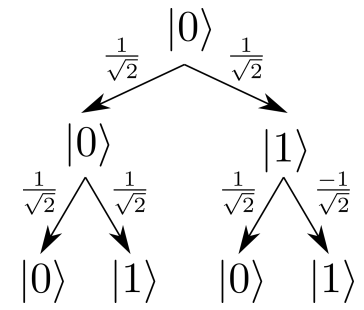
\includegraphics[width=0.3\textwidth]{qis001}
\end{center}

특정 경로의 진폭을 취하려면 그 경로를 따라 진폭의
곱을 취해야 한다. 특정 출력에 대한 마지막 진폭을 취하려면, 출력으로 이어지는
트리를 따르는 각 경로에 대해 진폭을 합해야 한다. 이 경우, $\ket0$의 진폭은 
$1$이고 $\ket1$의 진폭은 $0$이다. $\ket0$에 이르는 경로는 구성적으로 간섭하고,
$\ket1$에 이르는 경로는 파괴적으로 간섭한다.

\end{document}
